\documentclass[ngerman]{scrartcl}

\usepackage[utf8]{inputenc}
\usepackage{babel}
\usepackage[T1]{fontenc}
\usepackage{lmodern}
\usepackage{color}
\usepackage{graphicx}
\usepackage[colorlinks=true, linkcolor=cyan]{hyperref}
\usepackage{enumerate}
\usepackage{amsmath}
\usepackage{braket}
\usepackage{placeins}
\usepackage{amsfonts}

\newcommand{\erw}[1]{\langle {#1} \rangle}
\newcommand{\Hil}{\mathcal{H}}
\newcommand{\diff}{\mathrm{d}}

\usepackage[backend=bibtex, style=numeric-comp, sorting=nty]{biblatex}
\bibliography{mybib}

\begin{document}
 
	\begin{titlepage}
		\begin{minipage}[c][\textheight][c]{\textwidth}
			\begin{center}
				{ \Huge \textbf{Thermodynamik schwarzer Löcher} }
				
				\vspace*{1cm}
				{\large eine Seminararbeit von}
				
				\vspace*{0.2cm}
				{\Large Tamara Szecsey}
				
				\vspace*{1cm}
				{\large \today}
				
				\vspace*{4cm}
				\hspace*{1cm} 
\includegraphics[height=30ex]{LOGO_UR}
			\end{center}
		\end{minipage}
	\end{titlepage}
	
\tableofcontents
\newpage
\section{Einleitung}
Was ist Thermodynamik?

\section{Informationsentropie im Allgemeinen} \label{InfoentropieAllg}
Zunächst ein kurzer Einblick, um welche Art von Entropie es sich hier handeln wird. Ludwig Boltzmann hatte festgestellt, dass eine Proportionalität zwischen der Entropie $S$ und $\log W$ herrscht, wobei $W$ die Wahrscheinlichkeit darstellt. Der zugehörige Proportionalitätsfaktor $k$ ist die Boltzmann-Konstante.
	\begin{align}
		S &= k \log W
	\end{align}
Dies ist eine wichtige Verbindung zwischen Statistik und Thermodynamik. 
Die Verallgemeinerte Boltzmannsche Beziehung bring dann die sogenannte Informationsentropie hervor, die in diesen Gestalten geschrieben werden kann:	
	\begin{align} \label{Informationsentropie}
		S &=
		\left\{
		\begin{aligned}
		&- k ~\erw{\,\ln \rho\,} \\
		&-k~ Sp(\rho \ln \rho) \\
		&-k \sum_n \rho_n \ln \rho_n
		\end{aligned}
		\right.
	\end{align}
wobei $\rho$ die Wahrscheinlichkeit ist, die Energie $E_n$ im mikrokanonischen Ensemble anzutreffen. 
(Wir wollen hier nicht weiter auf die thermodynamische Definition der Entropie eingehen, für Fragen zu den Grundlagen siehe \cite{Brenig})

Wie wir jetzt aber zu Information kommen, soll ein Beispiel zeigen. Dabei geht es um eine quantitativen Betrachtung der selben.
Wir betrachten nun eine Reihe von Ereignissen $E_n (n = 1, 2, \ldots, N)$, die mit bestimmten Wahrscheinlichkeiten $\rho_n$ auftreten, wobei
	\begin{align*}
		\sum_{n=1}^N \rho_n &= 1
	\end{align*}
Nun sehen wir das Eintreten bestimmter die Ereignisse $E_n$, dabei hat jede unserer Feststellungen hat einen Informationswert $I_n$. Nach häufiger Wiederholung kann man einen mittleren Informationsgehalt aufstellen:
	\begin{align*}
		I = \sum_{n=1}^N \rho_n I_n
	\end{align*}
Hier legen wir wie in der Informationstheorie fest
	\begin{align*} \label{Informationsgehalt}
		I = - \sum \rho_n \mathrm{ld}(\rho_n)
	\end{align*}
wobei $\mathrm{ld}(x)$ der dyadische Logarithmus von $x$ ist, also $2^{\mathrm{ld}(x)} = x$. 
Wir haben \eqref{Informationsgehalt} so festgelegt, dass ein Ereignis allein durch eine Ja oder Nein Frage (oder durch 0 und 1) vollständig charakterisierbar ist. 
Dass unserer mittlerer Informationsgehalt unserer Entropie von \eqref{Informationsentropie} ähnlich sieht, ist kein Zufall.

Wir machen nun zwei Zahlenbeispiele zur Veranschaulichung:
	\begin{itemize}
		\item[\textit{1.\,Beispiel:}] Sei $N=2, \rho_1 = \rho_2= \frac{1}{2}$ was sein könnte: Ein Teilchen hält sich mit gleicher Wahrscheinlichkeit in der linken oder rechten Hälfe eines Kastens auf, oder Zahl und Wappen für ein Münzwurf.
		Es benötigt genau eine Ja-Nein-Frage, um herauszufinden, wo das Teilchen liegt oder wie herum die Münze gefallen ist.
			\begin{align*}
				I = \mathrm{ld}(2) = 1 \,\mathrm{bit}
			\end{align*}
		Ein Bit ist die Einheit für Information.
		\item[\textit{2.\,Beispiel:}]Sei $N=6, \rho_n = \frac{1}{6}$, wobei die Ereignisse $E_n$ die Seiten eines Würfels sein könnten, der Informationsgehalt
			\begin{align*}
				I = \mathrm{ld}(6) &= 2,58 \,\mathrm{bit}
			\end{align*}
	\end{itemize}
(siehe auch \cite{Brenig})

\section{In Bezug auf die thermodynamischen Hauptsätze}
	\subsection{Nullter Hauptsatz der Thermodynamik}
%Temperatur müssen wir definieren können
	Wir beginnen mit der Erklärung der Hawkingstrahlung. Diese fand Steven Hawking \cite{ParticleCreation}, als er den gekrümmten Raum in euklidische Koordinaten transformierte (z.B. Minkowski-Raum). Hierbei entstanden im Grundzustand Entartungen, die störungstheoretisch entwickelt werden müssen. 
	
	Anschaulich bedeutet dies, dass zwei verschränkte Teilchen (siehe Appendix \ref{Verschränkung}), die durch Vakuumfluktuation am Horizont des schwarzen Lochs entstehen so getrennt werden, dass das mit negativer Energie in das schwarze Loch hinein fällt, und das, welches eine positive Energie besitzt ins Unendliche im Raum verschwindet. 
	Genau letzteres sorgt für eine Hawkingstrahlung und die Hawkingtemperatur wie später in Kap \ref{evaporation} Gleichung \eqref{HawkingTemp} zu sehen.
	
	Nun besagt der nullte Hauptsatz der Thermodynamik, dass das schwarze Loch nur mit seiner Umwelt in thermodynamisches Gleichgewicht kommen kann, wenn es genauso viel Temperatur abstrahlt, wie es aufnimmt. 
	
	Dies hat eine Beschleunigung an der Oberfläche zum Mittelpunkt des schwarzen Lochs zur Folge. \marginpar{Bitte nochmal erklären}

	\subsection{Erster Hauptsatz der Thermodynamik}
%Innere Energie dU
	Der erste Hauptsatz der Thermodynamik besagt, dass die Änderung der inneren Energie gleich der Änderung der Wärme zusammen mit der Änderung der Arbeit ist, vorausgesetzt, es handle sich um ein geschlossenes System. Er steht somit für Energieerhaltung.
		\begin{align}
			\Delta U = \Delta Q + \Delta W
		\end{align}
	In unserem Fall wäre es nützlich, dies in der Form
		\begin{align}
			\diff E = T\diff S + \diff W
		\end{align}
	zu schreiben. 
	
	Tatsächlich findet man eine analoge Gleichung für schwarze Löcher.
	Dazu verwenden wir die zusammengedrückt Oberfläche mit einem ursprünglichen Radius gleich dem Schwarzschildradius, welche wie wir später abermals sehen werden, proportional zur Entropie ist (siehe Kap. \ref{zweiterHS}), welche durch die Kerr-Neumann Metrik und geschickt gewählten Koordinaten namens Boyer-Lindquist Koordinaten beschrieben wird. 
	\marginpar{bitte Referenz angeben}
	
	Da ich hier viele Formeln vermeiden möchte, bitte sehen Sie für Genaueres z.B. \cite{BekensteinHawking} oder \cite{Gebhardt}.
	
	Das Endergebnis ist von der Gestalt
		\begin{align} \label{1HS}
			\diff (Mc^2) = \frac{\kappa}{8 \pi G} \diff A + \Omega \diff J - \Phi \diff q
		\end{align} 
	Hier bei wurde $E = Mc^2$ benutzt, außerdem sind die zwei letzten Summanden der Drehimpuls und die elektrische Feldstärke. $\kappa$ ist auf dem Schwarzschildradius eine Konstante und wird allgemein als Oberflächen-Schwerebeschleunigung bezeichnet. (siehe \cite{Gebhardt})
	\\
	
	Dies bedeutet nun, dass die Änderung der Masse proportional zur Summe der Änderung der Fläche und der Änderung von Drehimpuls und elektrischem Feld ist. Es gilt also Massenerhaltung. \marginpar{stimmt das?}

\subsection{Zweiter Hauptsatz der Thermodynamik} \label{zweiterHS}
	Bevor man auf die obige Gleichung \ref{1HS} kommt, wird man feststellen, dass Masse, elektrische Ladung und Drehmoment in der gleichen Kombination immer proportional zur Oberfläche des schwarzen Lochs sind. 
	Außerdem haben sowohl Hawking \cite{ParticleCreation} also auch Misner, Thorne und Wheeler \cite{MisnerThorneWheeler} gezeigt, dass der Ereignishorizont eines schwarzen Lochs nicht kleiner werden kann, meistens wird er sogar größer. \marginpar{ich bin mir nicht immer ganz sicher in welchem Paper Hawking was gesagt hat}
	
	Diese Oberfläche verhält sich sozusagen wie die thermodynamische Entropie in geschlossenen Systemen. 
	
	Durch die Hawkingtemperatur und der Definition von Temperatur in der Thermodynamik
	\begin{align} \label{HawkingTemp}
	\frac{\diff S}{\diff E} &= \frac{1}{T},&
	T_{\text{Hawking}} &= \frac{\hbar c^3}{8 \pi G M}
	\end{align}
	und durch ersetzen von $E = Mc^2$, erhalten wir
	\begin{align} \label{BHentropie}
	S_{BH} &= \frac{c^3 A}{4 G \hbar} = \frac{A}{4 \ell_P^2} 
	\end{align}
	Der Horizont ist die1 Fläche $A$, welche eine Kugeloberfläche um das schwarze Loch mit dem Schwarzschildradius bildet:
	\begin{align} \label{OberflaecheSH}
	r_s &= \frac{2 GM}{c^2} ,& A = 4 \pi r_s^2 
	\end{align}
	Die Entropie in \eqref{BHentropie} wird auch Bekenstein-Hawking Entropie genannt. Die Plancklänge beträgt $\ell_p = \sqrt{\frac{G \hbar}{c^3}} \approx 10^{-32}\,$m.
	
	Ein sonnen-schweres schwarzes Loch hätte eine Horizontfläche $\frac{1}{5}$-mal so groß wie die Erdoberfläche und ihre Entropie wäre von der Ordnung $10^{77}$. Dies ist über zehn Größenordnungen höher, als die Entropie der jetzigen Sonne.  
	
	Es scheint also, dass die Entropie des schwarzen Lochs nicht mit der hineingefallenen Entropie während seiner Entstehung verglichen werden kann.
	
	Was man sich hier benützt, ist das sogenannte \textit{holographische Prinzip}.
	
\subsubsection*{Das holographische Prinzip}
	In einem flachen Raum, wie z.B. in der String Theorie verwendet, nehmen wir eine Region $\Gamma$ an, z.B. das Volumen ein schwarzen Lochs mit Radius gleich dem Schwarzschildradius. 
	Die maximale Entropie, also auch die maximale Information, welche in $Gamma$ hineinpasst ist proportional zur Fläche des Randes $\partial \Gamma$, in unserem Fall der Fläche A aus Gleichung \eqref{OberflaecheSH}.
	Dabei zählt die Entropie auf diesem Rand $\partial \Gamma$ in Planckflächen, genauer gesagt, ein Bit entspricht vier Planckflächen, anschaulich dargestellt in Abb. \ref{holoPrinzip}.
	\begin{figure} [h] 
		\begin{center}
			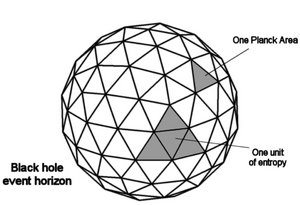
\includegraphics[width=0.6\textwidth]{BHentropy1}
		\end{center}
		\caption{Zweidimensionale Oberfläche des Horizonts aufgeteilt in Planck Einheiten. Die Entropie hat allerdings eine Einheit von 4 solchen Planckflächen für ein Bit. Siehe (\ref{BHentropie}). (aus \cite{BekensteinHawking})} \label{holoPrinzip}
	\end{figure} 
	
%zweiter HS Fläche proto Entropie, hier holographisches Prinzip
	Nun könnte man in einem Gedankenexperiment alle Energie und Information des Universums zusammenpacken, in ein solches Volumen und dann dieses soweit ausdehnen bis der Rand dieses Volumens der Rand des für uns sichtbaren Universums bildet. Alle Information, die es in unserem Universum gibt, wäre dann \textit{allein} in diesem Rand gespeichert!
%ganzes Universum, sehr verallgemeinert worden (Bousseau)
	
	Auf Grund des Oberflächen-Volumen Verhältnis (siehe Appendix \ref{O/V-Verhaeltnis}) ergibt sich, dass die Oberflächen zwei einzelner schwarzer Löcher immer kleiner ist, als die Oberfläche der bereits zu einem Dritten verschmelzen. Da wir inzwischen wissen, dass die Oberfläche proportional zur Entropie und diese wiederum proportional zur Masse des schwarzen Lochs ist, gilt 
		\begin{align}
			M_3 > M_2 + M_1
		\end{align} 
	wobei $M_3$ das verschmolzene schwarze Loch ist, welches ursprünglich mal aus $M_2$ und $M_1$ bestand. 
%bilder zwei schwarze löcher vereinigen M_3 > M_2 + M_1 usw.

\FloatBarrier
\section{Evaporation} \label{evaporation}

Wie wir bereits wissen, besitzt ein großes schwarzes Loch für einen Beobachter in großer Ferne eine Temperatur (siehe Gleichung \eqref{HawkingTemp}) besitzt. Dies hat eine Wärmestrahlung zur Folge also ein Energieverlust.

Dank Einstein wissen wir, dass Masse und Energie sich gleichen, wenn man c = 1 setzt. Jedes schwarze Loch verliert also im Lauf der Zeit an Masse, bis es verdampft. Dieser Vorgang wird als Evaporation bezeichnet. Nach einigen Rechnungen, siehe z.B. \cite{JerusalemsLectures}, erfahren wir, dass
	\begin{align}
		t_{\text{evap}} \sim G^2 M^3
	\end{align} 
Ein sonnenschweres schwarzes Loch würde nach etwa $10^{66}$ Jahren verdampft sein (zum Vergleich, das alter unseres Universums wird auf $13,8 \cdot 10^{9}$ Jahre geschätzt). Man hätte ein riesen Problem dies nachzuweisen, vielleicht wenn wir herausfinden, wie wir kleinere schwarze Löcher produzieren können. 

Aber was passiert mit der Entropie?
Hawking \cite{BreakdownGravitationalCollapse} legte dar, dass die Vorstellung, die Entropie würde die Anzahl der Möglichkeiten zählen, wie ein schwarzes Loch entstehen könne, gegen die Quantenmechanik verstößt.
Außerdem wird das schwarze Loch beim verdampfen bevor es komplett verschwindet erst Plancksche Größen annehmen, in der unsere bekannten physikalischen Gesetze vermutlich nicht mehr gelten. 

Eine von den zwei folgenden Ereignissen muss passieren:
	\begin{enumerate}[(1)]
		\item Die Verdampfung stoppt und das schwarze Loch in Planckgröße bleibt weiter unverändert im Raum. Dieses Überbleibsel hat eine sehr hohe Verschränkungsentropie weil es mindestens die gesamte Entropie des schwarzen Lochs vor dem Beginn der Verdampfung beinhalten muss. \label{1}
		
		\item Die Verdampfung wird zu Ende geführt. Die Energieerhaltung verhindert, dass mit dem letzten Ausstoß von Photonen genug Verschränkungsentropie mitgetragen werden kann, damit diese Zustände zusammen mit denen der zuvor ausgestrahlten Strahlung wieder einen reinen Zustand bilden können. Dies verletzt die Quantenmechanik, das Endresultat ist ein Mischzustand mit Entropie in der Größenordnung des Horizonts in Planckgrößen ganz am Anfang.  \label{2}
	\end{enumerate}
Punkt (\ref{1}) ist zwar Möglich, aber wenn ein schwarzes Loch aus Photonen und Gravitonen entsteht, dann muss es sich auch komplett wieder in diese auflösen können (es wäre also Inkonsistent mit der CPT(charge, parity, time = Ladung, Parität, Zeit)).

Unter Anderem Hawking plädieren für Punkt (\ref{2}). Er meint, dass die Entstehung und Verdampfung eines schwarzen Lochs nicht mit einer unitären S-Matrix beschrieben werden kann, also dass schwarze Löcher quantenmechanische und klassiche Information zerstören kann. 

Wem das nicht gefällt, der würde eher für einen dritten Punkt stimmen:
	\begin{enumerate}[(3)]
		\item Die Hawkingstrahlung kommt genau genommen nicht in einem Mischzustand. Die Information wird in den Verbindungen zwischen Hawkingphotonen hinausgetragen. Am Ende der Verdampfung haben wir wieder einen reinen Zustand des Strahlungsfeldes. Nur kleine Untersysteme sehen so aus, als wären sie thermisch, deshalb funktioniert diese Betrachtungsweise nur, wenn wir nicht auf zu viele Photonen zugleich schauen. 
	\end{enumerate}   
(Bei weiterer Interesse, bitte siehe Jerusalem Lectures \cite{JerusalemsLectures})
	
\section{Weitere Betrachtungen}
	\subsection{Wirkungsintegrale}
	Zur Berechnung der thermodynamischen Potentiale benötigt man in der Thermodynamik eine sogenannte Zustandssumme. Diese kann mit einem euklidischen Pfadintegral berechnet werden, welche alle möglichen Wege, die ein Teilchen einschlagen kann, unterschiedlich stark berücksichtigt. Deshalb ergibt sich aus der Summe aller gewichteten Pfade zwischen zwei Orten eine Gesamtwahrscheinlichkeit des Ortsübergangs.
	
	Die gesuchte Zustandssumme ist von der Gestalt 
		\begin{align}
			Z = \int \diff [\Phi] \exp \left(- \frac{I_E}{\hbar}\right) 
			\simeq \exp \left(- \frac{I_{E,B}}{\hbar}\right)
		\end{align}
	ist. Wobei $I_E$ die euklidische Wirkung ist, $\Phi(x,t)$ ist das Feld, welches wir betrachten. (für weiteres Verständnis siehe \cite{Gebhardt} und \cite{Pfadintegral})
	\marginpar{das elektrische Feld?}
	
	In Termen der höheren Ordnung entstehen Korrekturterme, welche die Fluktuationen der Felder und der  Metrik mit berücksichtigen.
	
	\subsection{Loop Quantum Gravity (LQG)}	%geht nicht in ART, CPT falsch
Die Loop-Quantengravitation (Loop = Schleifen) ist eine Konkurrenztheorie der Stringtheorie und nimmt keine Singularität in der Mitte des schwarzen Lochs an, sondern beinhaltet die Theorie, dass es weiße Löcher gibt, die sich wie schwarze Löcher verhalten, nur das die Zeit rückwärts läuft. 

Ein einlaufendes Wellenpaket würde dann, während es einem `Quantum bounce' (siehe Appendix
\ref{QuantumBounce}) durchmacht, durch das schwarze Loch in ein weißes Loch hineintunneln. Eine Metrik dazu haben Rovelli und Haggard \cite{LQGRovelli} aufgestellt. Die Folge für die Entropie des schwarzen Lochs sind am Ende `nur' Korrekturterme.
%Hier kommen damit korrekturen 

%nur Quantenmechanik sagen, Information kann nicht verloren geht

\appendix
\section{Zustände in der Thermodynamik}

\subsection*{Mikrozustand}
Ein Mikrozustand ist im klassischen Fall ein Punkt im Phasenraum. Damit ist Ort und Impuls für jedes Teilchen gegeben.

\subsection*{Makrozustand}
Viele Mikrozustände bilden einen Makrozustand, der durch Parameter dargestellt ist, die nicht mehr direkt mit Ort oder Impuls einzelner Teilchen zu tun hat.

\section{Verschränkung} \label{Verschränkung}
	Durch die Quantenfluktuation im Vakuum, die durch die Heisenbergsche Unschärferelation auch erlaubt ist, können Teilen und Antiteilchen für kurze Zeit sozusagen aus dem Nichts entstehen und wieder verschwinden. Dabei sind genau diese Teilen verschränkt.
	\\ \\
	Was das genau bedeutet erkläre ich nun Anhand eines einfacheren Beispiels:
	
	Sagen wir, wir besitzen zwei Kugeln, welche die Farben blau oder rot haben können. Sie können allerdings nicht die gleiche Farbe haben. 
	Zu Beginn wissen wir nicht, welche Kugel welche Farbe hat, sie stecken z.B. in zwei separaten Kisten. Wir nennen die Kugeln $K_1$ und $K_2$ und entfernen Sie voneinander, sodass wir nur noch $K_1$ in einer Kiste vor uns haben. 
	
	Wenn wir nun die Kiste öffnen, wissen wir nicht nur, welche Farbe $K_1$ hat, sondern auch, dass die Kugel $K_2$, die wir im Moment nicht sehen können, genau die andere Farbe hat! 
	Solange wir aber die Kisten nicht öffnen, befinden sich die Kugeln in einem verschränkten Zustand, in dem zwar beide Farben möglich sind, aber die Farben voneinander abhängen. 
	
	Das bedeutet allerdings nicht, dass so Information übertragen werden kann. Entfernen wir z.B. die zweite Kugel bis zum anderen Ende der Milchstraße, so wissen wir beim Öffnen unserer Kiste welche Farbe die Kugel auf am anderen Ende hat, aber die Person, die dort steht wird das erst erfahren, wenn sie selbst die Kiste öffnet oder wir ein Signal dort hingeschickt haben.

\section{Quantum bounce} \label{QuantumBounce}
	Wenn es z.B. um die Urknalltheorie geht, dann besagt der Quantum bounce, dass unser Universum erst ausgedehnt war wie es jetzt ist, dann sich der Raum sehr hoch verdichtet hat, und dann wieder in die jetztige Größe `gebounct' ist. Das bedeutet im Falle der LQG, dass das schwarze Loch sich irgendwann zusammenzieht, und dann als weißes Loch wieder `zurückbounct' und sozusagen alles, was es aufgesaugt hat, wieder ausspuckt. Da aber für einen entfernten Beobachter Gegenstände, die Nahe am Horizont sind und gerade hineinfallen, unglaublich langsam erscheinen, wird es sehr lange dauern, so einen 'Quantum bounce' bei einem schwarzen Loch zu sehen.  

\section{Oberflächen-Volumen Verhälnis} \label{O/V-Verhaeltnis}
	Das Volumen einer Kugel steigt im Verhälnis zu ihrer Oberfläche nur zu einem Drittel.
	Das kann man so berechnen
		\begin{align*}
			\left.
			\begin{aligned}
			A &= 4 \pi r^2 \\
			V &= \frac{4}{3} \pi r^3 
			\end{aligned}
			\right\}
			&\Rightarrow 
			\frac{A}{V} = \frac{4 \pi r^2}{\frac{4}{3} \pi r^3} = \frac{3}{r} \\
			\text{setzte }r = 1 &\Rightarrow V = \frac{1}{3} A			
		\end{align*}
	Ein ähnliches Verhältnis gilt für alle Körper. In der Biologie versucht man so zu erklären, warum die Menschen in kalten Regionen im Durchschnitt größer sind als in warmen. 
\newpage
\printbibliography
%\printindex
%@article{Mukhanov,
%AUTHOR = {Mukhanov, V.F.}
%JOURNAL = {Foundations of Physics},
%Volume = 33,
%Pages = 271,
%YEAR = 2003
%}
%@article{Srednicki,
%	AUTHOR = {Srednicki, M.},
%	JOURNAL = {Class. Quantum Gravity},
%	Volume = 71,
%	Pages = 66,
%	YEAR = 1993,
%	URL = {http://xxx.lanl.gov/abs/hep-th/9303048}
%}
%@article{StromingerWafa,
%	AUTHOR = {Strominger, A. and Wafa, C.},
%	JOURNAL = {Physics Letters B},
%	Volume = 379,
%	Pages = 99,
%	YEAR = 1996,
%	URL = {http://xxx.lanl.gov/abs/hep-th/9601029}
%}
%@article{FrolovNovikov,
%	AUTHOR = {Frolov, V. and Novikov, I.},
%	TITLE = {Dynamical Origin of the Entropy of a Black Hole},
%	JOURNAL = {Physical Review D},
%	YEAR = 1993,
%	VOLUME = 48,
%	PAGES = 4545,
%	URL = {http://xxx.tau.ac.il/abs/gr-qc/9309001}
%}
%@article{BombelliKouLeeSorkin,
%	AUTHOR = {Bombelli, L., Koul, R., Lee, J. and Sorkin, R.},
%	JOURNAL = {Physical Review D},
%	Volume = 34,
%	pages = 373,
%	year = 1986,
%	URL = {http://dx.doi.org/10.1103/PhysRevD.34.373}
%}
%@article{BowickSmolinWijewardhana,
%	AUTHOR = {Bowick, M., Smolin, L. and Wijewardhana, L.C.R.},
%	JOURNAL = {Gen. Rel. Grav.},
%	VOLUME = 19,
%	PAGES = 113,
%	YEAR = 1987
%}
%@article{Carlip,
%	AUTHOR = {Carlip, S.},
%	JOURNAL = {Class. Quantum Gravity},
%	Volume = 16,
%	Pages = 3327,
%	YEAR = 1999,
%	URL = {http://xxx.lanl.gov/abs/gr-qc/9906126}
%}
%@article{Wald,
%	AUTHOR = {Wald, R.M.},
%	JOURNAL = {Physical Review D},
%	Volume = 48,
%	Pages = 3427,
%	YEAR = 1993,
%	URL = {http://xxx.lanl.gov/abs/gr-qc/9307038}
%}
%@article{Witten,
%	AUTHOR = {Witten, E.},
%	JOURNAL = {Advances in Theoretical and Mathematical Physics},
%	Volume = 2,
%	Pages = 253,
%	YEAR = 1998,
%	URL = {http://xxx.lanl.gov/abs/hep-th/9802150}
%}
%@article{ThorneZurek,
%	AUTHOR = {Thorne, K. S. and Zurek, W. H.},
%	JOURNAL = {Physical Review Letters},
%	Volume = 54,
%	Pages = 2171,
%	YEAR = 1985,
%}
%@article{Susskind,
%	AUTHOR = {Susskind, L.},
%	TITLE = {Some speculations about black hole entropy in string theory},
%	JOURNAL = {unpublished},
%	YEAR = 1993,
%	URL = {http://xxx.lanl.gov/abs/hep-th/9309145}
%}
%@article{Hooft,
%	AUTHOR = {'t Hooft, G.},
%	JOURNAL = {Nuclear Physics B},
%	Volume = 256,
%	Pages = 726,
%	YEAR = 1985,
%	JOURNAL = {International Journal of Modern Physics A},
%	Volume = 1,
%	Pages = 4623,
%	YEAR = 1996,
%	URL = {http://xxx.lanl.gov/abs/gr-qc/9607022}
%}
\end{document}